  \documentclass[a4paper, titlepage]{report}
\usepackage[utf8]{inputenc}
\usepackage[T1]{fontenc}
\usepackage[french]{babel}

\usepackage{graphicx} 


\usepackage{lmodern} % Pour changer le pack de police
\usepackage[vlined, longend]{algorithm2e}
\usepackage{multicol}
\usepackage[a4paper, top=2cm, bottom=2cm, left=2cm, right=2cm]{geometry}


\usepackage{wrapfig}
 


\setlength{\algomargin}{0em}
\SetKwRepeat{Repeat}{Do}{While}
\SetKwIF{If}{ElseIf}{Else}{If}{then}{Else if}{Else}{EndIf}
\SetKwFor{For}{For}{do}{Done}
\SetKwFor{While}{While}{do}{Done}

\providecommand{\SetAlgoLined}{\SetLine}
\providecommand{\DontPrintSemicolon}{\dontprintsemicolon}

\SetKwBlock{Begin}{Begin}{End}

\SetKw{KwFrom}{from }
\SetKw{KwBy}{by }
\DontPrintSemicolon	% do not print the ';' symbol
\newcommand{\TRUE}{\textit{TRUE} }
\newcommand{\FALSE}{\textit{FALSE} }
\newcommand{\AND}{\textit{AND} }
\newcommand{\OR}{\textit{OR} }
\newcommand{\NULL}{\textit{NULL} }

\newcommand{\NewWhile}{\SetKwBlock{While}{while}{}}
\newcommand{\NormalWhile}{\SetKwBlock{While}{while}{Done}}

\setcounter{secnumdepth}{5}
\setcounter{tocdepth}{5}

\newenvironment{lexicon}{\noindent \hspace{1.2em} {\bf \underline{Lexicon}} \\~\\}{ ~\\ }
\newenvironment{algo}{\noindent \hspace{1.2em} {\bf \underline{Algorithm}} \\~\\ \begin{algorithm}[H] \SetAlgoLined }{\end{algorithm}  ~\\}

\usepackage{listings}
\lstset{ 
language=java
}

\title{LO43 
     Flotte de véhicules autonomes}
\author{Buri Theo florian Lacour} 
\date{Hiver 2013}

\makeatletter
\def\clap#1{\hbox to 0pt{\hss #1\hss}}%
\def\ligne#1{%
\hbox to \hsize{%
\vbox{\centering #1}}}%
\def\haut#1#2#3{%
\hbox to \hsize{%
\rlap{\vtop{\raggedright #1}}%
\hss
\clap{\vtop{\centering #2}}%
\hss
\llap{\vtop{\raggedleft #3}}}}%
\def\bas#1#2#3{%
\hbox to \hsize{%
\rlap{\vbox{\raggedright #1}}%
\hss
\clap{\vbox{\centering #2}}%
\hss
\llap{\vbox{\raggedleft #3}}}}%
\def\maketitle{%
\thispagestyle{empty}\vbox to \vsize{%
\haut{}{\@blurb}{}
\vfill
\vspace{1cm}
\begin{flushleft}
\usefont{OT1}{ptm}{m}{n}
\huge \@title
\end{flushleft}
\par
\hrule height 4pt
\par
\begin{flushright}
\usefont{OT1}{phv}{m}{n}
\Large \@author
\par
\end{flushright}
\vspace{1cm}
\vfill
\vfill
\bas{}{\@location, \@date}{}
}%
\cleardoublepage
}
\def\date#1{\def\@date{#1}}
\def\author#1{\def\@author{#1}}
\def\title#1{\def\@title{#1}}
\def\location#1{\def\@location{#1}}
\def\blurb#1{\def\@blurb{#1}}
\date{Décembre 2014}
\author{}
\title{}
\makeatother
\title{LO43 Flotte de véhicule autonomes}
\author{Buri Theo Florian Lacour}
\location{Belfort}
\blurb{%
Université de technologie de Belfort-Montbéliard
}% 

\usepackage{array}


\begin{document}


\maketitle
\tableofcontents
\newpage
\chapter*{Introduction}
\addcontentsline{toc}{chapter}{Introduction}
\hspace{0.5cm}Dans le cadre de  l'UV LO43 " Bases fondamentales de la programmation orientée objet", il nous a été demandé de réaliser un projet de groupe, afin de mettre en pratique les connaissances acquises lors des cours et TDs du semestre.
\\
Trois sujet nous on été présentés. Nous avons fait le choix de traiter le sujet de la "Flotte de véhicules autonomes", et ceci pour plusieurs raisons :
\begin{itemize}
  \item (A TROUVER)
  \item N'étant que deux, sur un maximum de quatre étudiants par groupe autorisés, les autres sujets ne nous ont pas parus réalisables en temps et en heures et sans bugs majeurs...
  \item (A TROUVER)
\end{itemize}
Nous présenterons tout d'abord le sujet, ses contraintes, et les libertés prises par rapport à celles-ci. Par la suite, nous parlerons des différents diagrammes UML, et les expliquerons. Enfin, nous terminerons par l'implémentation en Java et l'interface graphique.


\setcounter{chapter}{1}
\setcounter{section}{1}
\part{ Présentation du sujet}
\section{Objectif}
 Le programme à réaliser consistait en la modélisation d'une flotte de véhicules évoluant dans une infrastructure de circulation partagée. Pour cela, il a tout d'abord fallu modéliser la partie calculatoire à l'aide du langage UML, puis ensuite l'implémenter en Java et lui donner une interface graphique
\section{Reformulation du sujet}
\subsection{Plateau}
Le plateau donné par le sujet est le suivant :
\vspace{0.5cm}

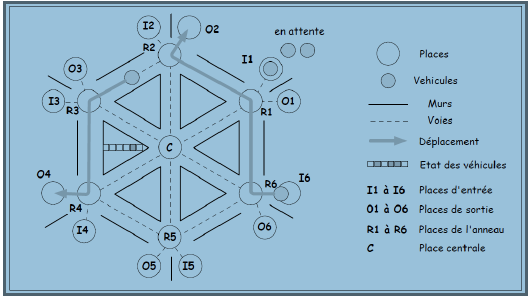
\includegraphics[]{Images/Plateau}
\vspace{0.5cm}
\\
Chaque place, exceptée celle du centre, est rattachée à une place de départ et une place de sortie. Les voitures disposant d'une mission partent depuis une place d'entrée et, à la fin de celle-ci, rejoingent une place de sortie.\\
La place centrale n'est utilisée que lors d'un trajet reliant deux places opposées...
\subsection{Missions et contrôleur}
Chaque passager doit être transporté d'une place à une autre. Pour ce faire, ils envoient une requête au module qui se charge du contrôle du plateau : le contrôleur. Par la suite, celui-ci assignera cette mission à un des véhicules de sa flotte. Celui-ci calculera ensuite le trajet qu'il suivra pour la mener à bien.\\
C'est alors le véhicule qui décide de partir : pour cela il doit envoyer une requête au contrôleur pour savoir si son chemin est déjà réservé. Si ce n'est pas le cas, le contrôleur l'autorise, et le véhicule part. La requête se fait sous la forme d'une Request Map, constituée de booléens indiquant l'intention du véhicule de réserver une place ou non.\\
Pour exemple, lorsqu'une voiture désire aller de la place I1 à O2, elle aura besoin de réserver I1, R1, R2 et O2. La Request Map seras alors la suivante :
\vspace{0.5cm}

\begin{tabular}{|l|l|l|l|l|l|l|l|l|l|l|l|l|l|l|l|l|l|l|l|}

\hline
  I1 & I2 & I3 & I4 & I5 & I6 & R1 & R2 & R3 & R4 & R5 & R6 & O1 & O2 & O3 & O4 & O5 & O6 & C \\
  \hline
   T & F & F & F & F & F & T & T & F & F & F & F & F & T & F & F & F & F & F\\
 \hline

\end{tabular}\\
\vspace{0.25cm}\\
Afin d'éviter toute erreur lors de la réservation, nous avons défini la priorité des places qui suit:
\begin{center}
I1<I2<I3<I4<I5<I6<R1<R2<R3<R4<R5<R6<O1<O2<O3<O4<O5<O6<C
\end{center}
Ceci permettra d'éviter que deux véhicules tentent de réserver la même place à deux moments différents, et que le contrôleur les valide...

\subsection{Contraintes et libertés prises sur le sujet}


S'ajoutent alors quelques contraintes, qui régissent le programme :
\begin{itemize}
  \item Les véhicules ne peuvent utiliser la place centrale qu'à la seule condition qu'ils doivent se rendre à la place en face de la leur.
  \item Une place ou une route (reliant deux places) ne peut être utilisée que par un seul et unique véhicule.
  \item Un véhicule qui souhaite emprunter un chemin occupé doit attendre que celui-ci se libère.
\end{itemize}
\vspace{0.25cm}
Ainsi, par rapport à ces différentes consignes, nous avons choisi de prendre certaines libertés :
\vspace{0.25cm}
\begin{itemize}
  \item Un véhicule ne peut pas contourner une place occupée pour mener sa mission à bien.
  \item 
\end{itemize}
\part{Conception UML}
%non de chapitre a changer
\chapter{Les Diagramme UML}
\section{Diagramme des cas d'utilisation (annexe A)}
\hspace{0.5cm} Le diagramme des cas d'utilisation permet de représenté les action que l'utilisateur peut faire. Dans notre projet, en lançant le jeux l'utilisateur a plusieurs solution:
\begin{itemize}
\item voir les crédit.
\item Choisir de jouer en mode manuel, dans ce cas il devras après choisir le chemin de la voiture
\item Jouer en simulation, dans ce mode toute les requête sont générer par le programme
\item axé aux option, une fois dans ce menus, il peut choisir de changer les graphique du jeu, il peut aussi changer la rapidité des voitures.
\end{itemize}
\section{Diagramme de sequence(annexe B)}
\hspace{0.5cm} Le diagramme de séquence permet de représenté les interaction entre les différentes classes selon un ordre chronologique.
\section{Diagramme de classes(annexe C)}
\hspace{0.5cm} Nous verrons en détail, une description de chaque classe.
\chapter{Description des classes}
\section{Classe BoiteAuxLettre}
   \begin{minipage}{0.49\textwidth}
       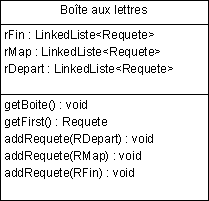
\includegraphics[scale=1]{Images/BoiteAuxLettre.PNG}
    \end{minipage}
    \begin{minipage}{0.49\textwidth}
      Il s'agit de la classe recevant toute les requêtes, qu'elle soit envoyer de la partie graphique, ou du modèle. Il y a 3 requête:
      \begin{itemize}
      \item Une liste de requête de départ cette liste contient toute les demande de trajet. Ces trajet peuvent être demander soit par l'utilisateur, soit générer par le modèle.
      \item une liste nommé rMap, ce sont les requête qu'envoies chacun de véhicule pour demander si leurs route sont libre ou non.
      \item rFin, ce sont les requête qu'envoies touts les véhicules lorsqu'ils ont terminer leurs trajets. Elle permettent de libérer toutes les routes 
      \end{itemize}
      La méthode getFirst() renvoi une requête celons un ordre de priorité. En effet dans un premier temps elle renverras une requête de fin de trajet afin que les trajet soit libérer le plus vite possible. Puis nous regardons si il y a une requête de Depart, afin que la liste de véhicule désirant partir soit le plus complet possible
    \end{minipage}
    
%  les annexes
\appendix
%diagrame cas d'utilisation
\chapter*{Annexe A}
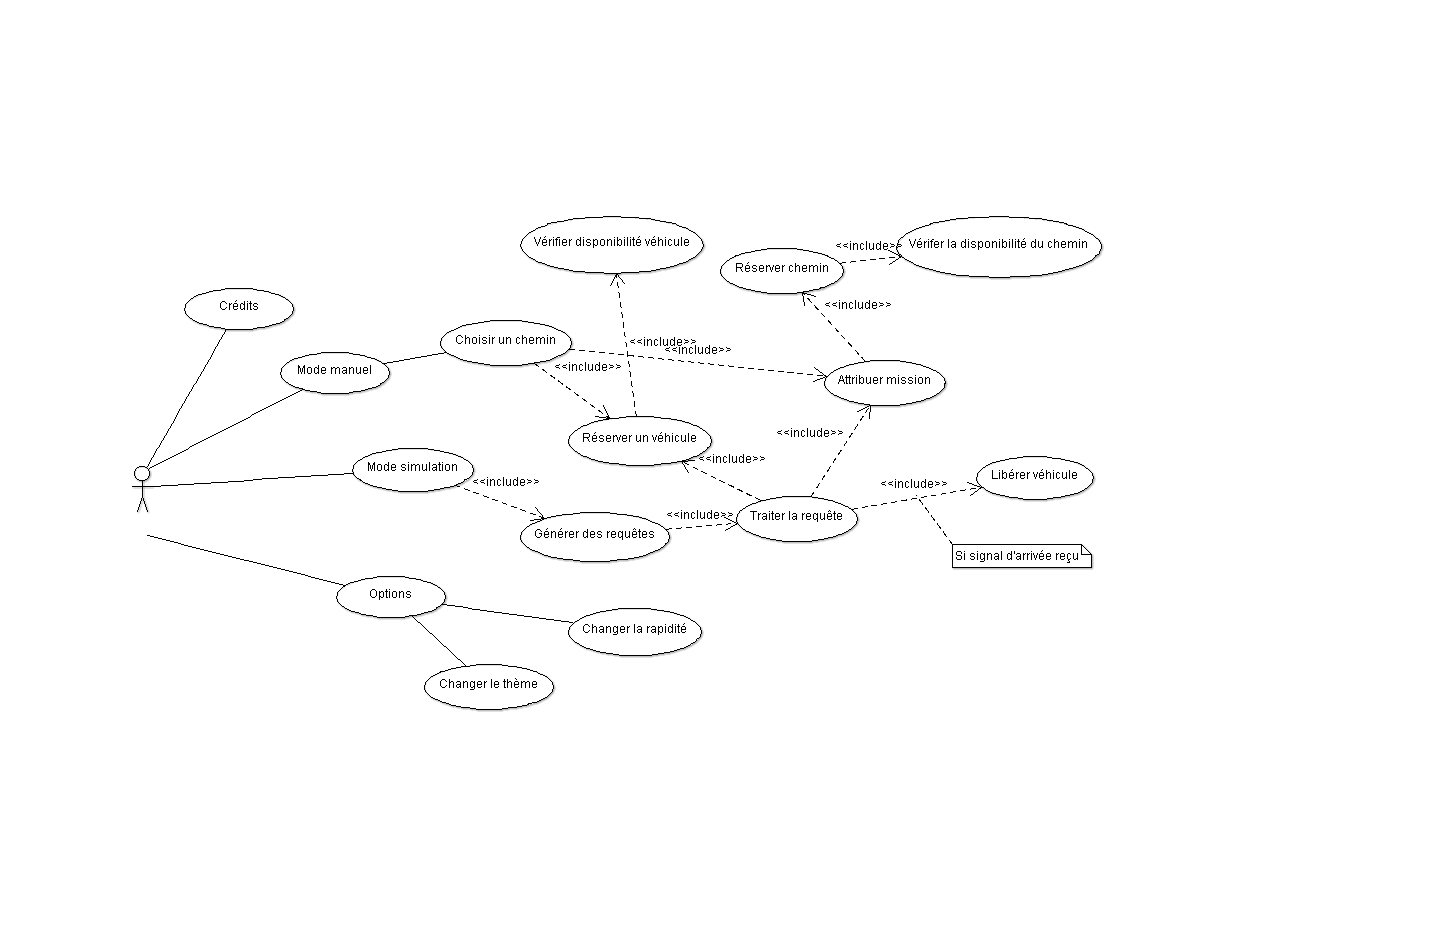
\includegraphics[width=20cm, height=15cm]{Images/CasUtilisation.PNG}
%diagrame de sequence
\chapter*{Annexe B}
\end{document}